\section{Using the LCD screen}


\textbf{LCD Usage}

When initially deciding to use the LCD, we knew we would have problems with it.  The LCD's are known to be difficult in setting it up to do what you want and there was no sample code for us to look at or use as a reference. To get the LCD to work, we would have to make the setup code and the code for printing to the screen ourselves. This was the hardest part of the code  in terms of thinking required. We would have to know what all the pins are and what port we would use on the AVR. Then we would also need to know the proper instructions for setting up the LCD.

\textbf{LCD Wiring}

Initially, we realized that the LCD had 16 pin inputs but the datasheets we found said that there were only 14 pins used. I looked at the bottom of the LCD and found there to 14  lines coming from the input headers. This lead me to calling these pins the 14 we would use; these pin numbers were 1 – 13 and 15. The first three pins are strictly analog circuitry. Pin  1 is just the ground and Pin  2 was the  the power supply (5V). The third pin is just for the contrast of the LCD where higher voltage would lighten the screen and ground would make it display at its greatest contrast. The next three pins were for setting up the commands for the LCD. These pins were set to use the 3 most significant bits (MSB) of PORT B, with the other half used by the circuitry for the multimeter. The last 8 bits were connected to PORT D which we hadn't used yet. These bits will also be for transmitting commands, primarily characters. 
	Wiring notes provided by the datasheet can be seen below.

\begin{figure}[h]
\centering
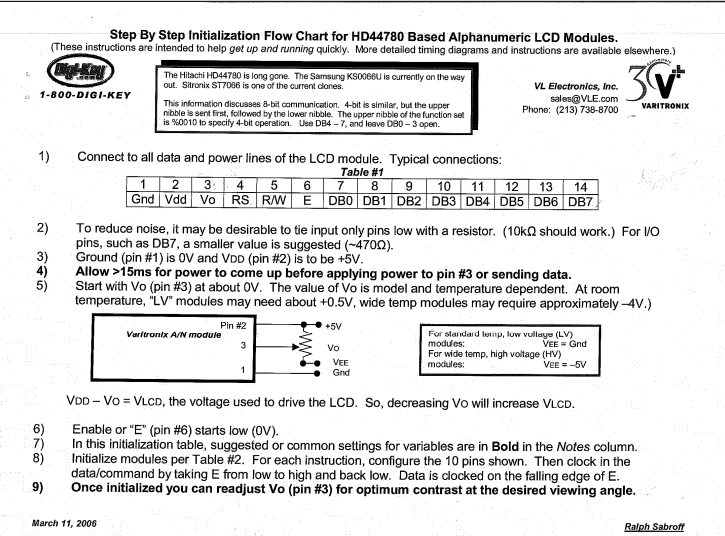
\includegraphics[width=0.8\textwidth]{screenshot6}
\caption{Initialization Instructions 1}
\label{SECTION:fig:IFC}
\end{figure}

\subsection{LCD Initialization}
For initializing the LCD, we found a generic Hitachi HD44780 type initialization instruction set. The basic idea is this:

\begin{itemize}
\item Setup the display type
\item Setup the display type\begin{itemize}
\item Choose the desired display type
\item Number of bits that will be sent at once
\end{itemize}
\item Clear the Display
\item Choose enter mode \begin{itemize}
\item Print left to right of right to left
\item shift the display?
\end{itemize}
\item Choose display \begin{itemize}
\item Want the display on?
\item Want a cursor?
\item What the characters to blink?
\end{itemize}
\end{itemize}

\begin{figure}[h]
\centering
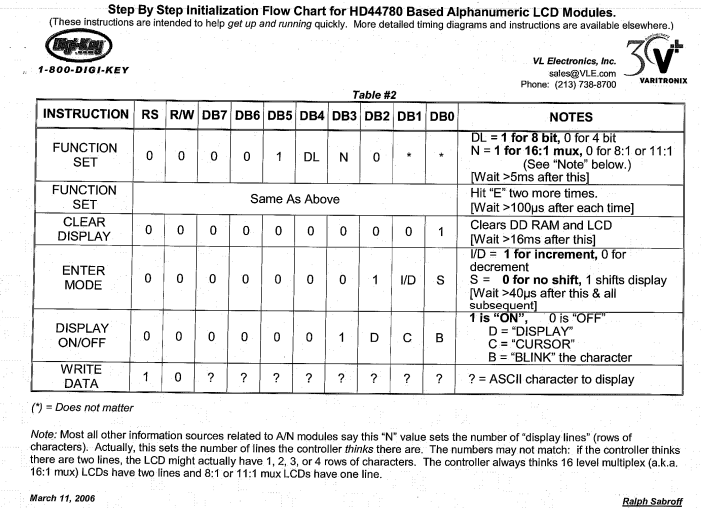
\includegraphics[width=0.8\textwidth]{screenshot7}
\caption{Initialization Instructions 2}
\label{SECTION:fig:funcset}
\end{figure}

For our setup, we decided to go with a 16:1 display type sending 8 bits at once. The display would print left to right without shifting the display; it would also show a cursor with no blinking. We decided on the 16:1 mux because that is the only setup our LCD would properly display, and we chose the 8 bits setup because this would make sending characters really simply. Display characters left to right made the most sense to us since we weren't writing in katakana and this is a numeric display. Cursors are nice to look at so, why not have one, right? 

A key note in this section is the time delay. It is crucial that the timing of sending the commands by setting the enable or 'E' bit from low to high and than back to low via our function EHIT() be more than the limits given. For safety reasons, in terms of the time delay, we set the delays to be much greater than necessary. This make sure that everything is sent to the LCD correctly add not too fast. On the down side however, the LCD is noticeably slower. For the time delays we use the \_delay\_ms() functions found in utils/delay.h . Initially, we used a simple for loop type but thought this was not really a robust way of doing it.  Attached to this report is the code for initialization of the LCD.

\subsection{Printing to the LCD}

To  print to the LCD, we used a similar setup as we had used in the previous labs where we printed strings to the serial connection. Instead of sending it to the UDR, we send each character one at a time to the LCD via PORT D. In order to print strings, we will once again incorporate sprintf() so as to create an array of characters that can be passed to the printLCD() function we created. The only problem with this printing, is that only the first 8 display addresses on the LCD are used. This means we cannot print any strings longer than 8 characters not including the null terminating character. This however, may be a problem with the LCD initialization rather than the printLCD(). The code for the printLCD function is relatively short and is attached last in the report.

\subsection{Problems with the LCD}

\textbf{Rewiring the LCD}

After writing the code, we test the LCD by just having it print the character 'a' after initialization. This yielded no results. Using deduction, we determined that the problem lay in the initialization code. After making the code more accurate and fixing a lot of little bugs we missed, like correctly masking the 3 MSB in PORT B so as not to interfere with the voltmeter stuff., we were still failing to initialize the LCD. After spending well over a day on initialization code editing, it was brought to our attention, that there were really 16 connections to the LCD header rather than 14 as we initially thought. After some  contemplation, we referred to Andy Sheaff as he has plenty of experience with these LCD's and others of the same type and is responsible for getting these to work for the PIC chips used in ECE 177.  He informed us that the last two pins were just for the backlight and that these models, though providing the pins, do not have a backlight. These two lines can be seen coming from the 15th and 16th pins of the LCD. This meant that something was wrong with what I saw on the bottom. Looking at the bottom again, I discovered that the line coming from what I thought to be Pin 15 was actually Pin 14. After this small rewiring task, the initialization worked just as it was designed to.

\textbf{The Biggest Problem}

To be short and sweet about this note, we decided to debug the printLCD function by having the AVR print to the computer via the serial connection and minicom and then print the same characters to the LCD. This resulted in “garbled” characters and the loss of 2 1/2  days trying to recode the printLCD and lcd\_init functions. When we finally realized that the problem was our TX and RX lines were off the pins we were using as PORT B,  we knew all we had to do was just use the LCD and forget about debugging using the serial connection. After getting rid of the serial communication, our LCD initialization and printing code worked like it was supposed to. If we had taken the time to look at the entire wiring of the circuit we would have probably realize these two mistakes and saved ourselves days of debugging the LCD that could have been allocated to the actual multimeter and the A-D converting.